The system implementation is divided into four main modules, Feature extraction, Pose estimation, Non-linear optimization and 3D visualization.

\begin{figure}[htb]
	\centering
	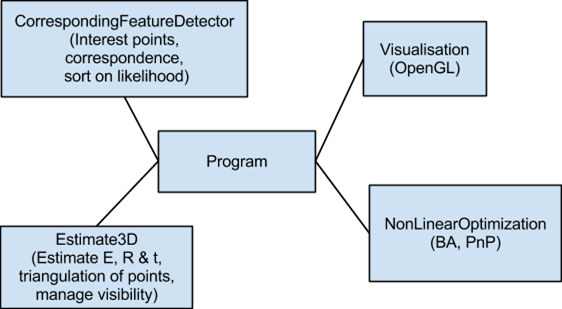
\includegraphics[width=110mm]{images/system_modules.png}
	\caption{\textit{Modules of the system}}
	\label{fig:block_overview2_fig}  %Skapar referens till figuren
\end{figure}

First feature extraction using Harris is performed as a preprocessing step on all images. These are used to calculate pairwise image point correspondences using SIFT.

Then an iterative process is performed cycling though all camera-pairs, each consisting of two parts. The first part contains an initial camera pose estimation, of the new camera, using the essential matrix estimated from F using the Gold standard algorithm. The camera pose is then improved using PnP on all previously known 3D-points and over all cameras. An initial 3D-point triangulation is then calculated.
The second part is a bundle adjustment over all current 3D points and cameras by the means of a non-linear optimization.

When all camera poses and estimated 3D-points have been iteratively added and optimized the result is rendered using OpenGL.

\begin{figure}[htb]
	\centering
	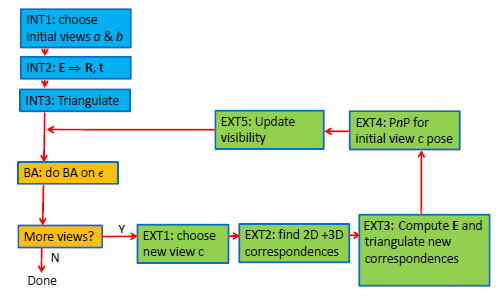
\includegraphics[width=120mm]{images/data_flow.png}
	\caption{\textit{Data flow between modules.}}
	\label{fig:block_overview_fig}  %Skapar referens till figuren
\end{figure}
